\subsection{Horizontal velocity (ice flow)}

\begin{figure}[H]
    \centering
    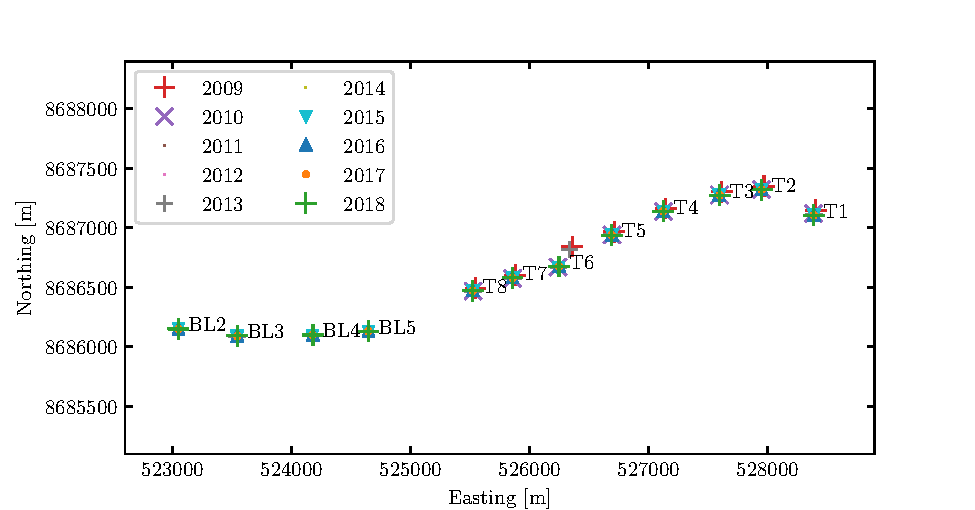
\includegraphics[width=\textwidth]{./figs/stakePositions.pdf}
    \caption{Positions of all stakes in the flow line on Blekumbreen and Tellbreen.
    The different markers distinguish the year of the measurement.}
    \label{GPS:fig:stakepos}
\end{figure}

Figure~\ref{GPS:fig:stakepos} shows the positions of the currently 12 different stake locations
on Blekumbreen and Tellbreen.
At those locations, a total of 26 measurements has been performed in 2018.
Additionally, all available data of the stake positions since 2009 is shown on the figure.

The coarse resolution of the figure shows a rough accordance of all of this years positions with the values 
of the last years.
The stakes spread over about 5 kilometers in east-west direction and 1.5 kilometers in north-south direction.


Figure~\ref{GPS:fig:T1_2d} shows all available data for T1 in a higher resolution.
The measurement of the location of T1-2017 (green) has been performed two times in order to estimate the uncertainty
of the position.
The two positions differ by 19\,cm and match within their uncertainties.

Equation~\ref{GPS:eq:v} shows how the ice velocity $v_{year}$ has been calculated with the measured stake positions from
Tab.~\ref{GPS:tab:os_tab}:
The distance between this years position and the position measured in 2017, 2016 or 2015 has been divided by the time $t$
(one, two or three years).
$N_{year}$ and $E_{year}$ are the northing and easting of the year which has been used to calculate the distance to
this years position.
The positions of this year ($N_{year, 2018}$ and $E_{year, 2018}$) have been shifted by the respective distance
$\Delta_{\text{ref}, year}$ that ablation has
added to an inclined stake since the year $year$, as described in section~\ref{GPS:sec:Processing}.
Equation~\ref{GPS:eq:sv} shows how the error on $v_{year}$ has been obtained.

Table~\ref{GPS:tab:vel_tab} lists the calculated velocities for all stakes.
The direction of the movements can be seen on the detailed figures for each stake in the appendix.


\begin{figure}[H]
    \centering
    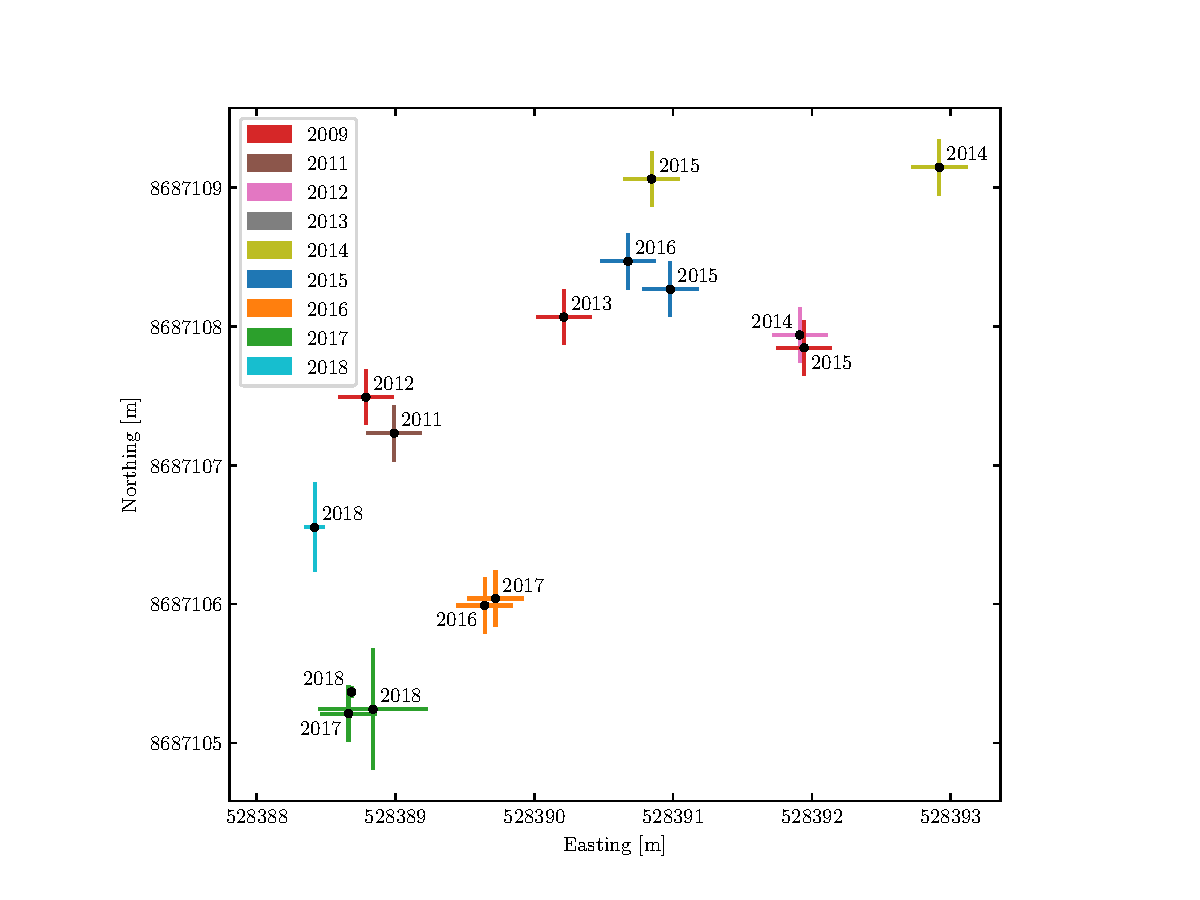
\includegraphics[width=\textwidth]{./figs/T1_2d.pdf}
    \caption{Measured positions at the location of stake T1 from 2011 to 2018.
    Different colors denote different stakes;
  	the year next to each stake position is the year of the measurement.
  	The measurements of 2018 have been corrected by the inclination of the stake and
  	the distance between the stake and the rover, therefore the coordinates refer to the intersection point
  	of stake and glacier surface.
    	At this location, a movement in south-east direction would be expected.
    	This is not identifiable using the data at hand.
 	Similar plots of the other 11 stake locations are situated in the appendix.}
    \label{GPS:fig:T1_2d}
\end{figure}


\begin{table}[h]
	\caption{Velocities of the stakes measured in 2018, calculated with equations~\ref{GPS:eq:v} and \ref{GPS:eq:sv}.
	The velocity $v_{2017}$ has been calculated using last years position
	For inclined stakes, this position has been corrected for the horizontal displacement due to ablation.
	If available, corrected positions from 2016 and 2015 have also been used to obtain $v_{2016}$ and $v_{2015}$.
	To be able to assess the uncertainty of the velocities, four measurements have been performed twice.
	This is denoted by the suffices -i and -ii.}
	\centering
	\begin{tabular}{lcccccc}
\toprule
  Stake name & Velocity (2017) [m/a] & Velocity (2016) [m/a] & Velocity (2015) [m/a] \\
\midrule
    BL2-2016 &       0.26 $\pm$ 0.21 &       0.21 $\pm$ 0.20 &                     - \\
    BL3-2016 &       0.16 $\pm$ 0.20 &       0.21 $\pm$ 0.18 &                     - \\
  BL4-i-2016 &       0.07 $\pm$ 0.26 &       0.08 $\pm$ 0.25 &                     - \\
 BL4-ii-2016 &       0.11 $\pm$ 0.56 &       0.05 $\pm$ 0.48 &                     - \\
  BL5-i-2017 &       1.75 $\pm$ 0.18 &                     - &                     - \\
 BL5-ii-2017 &       1.74 $\pm$ 0.24 &                     - &                     - \\
   T1-i-2017 &       0.09 $\pm$ 0.11 &                     - &                     - \\
  T1-ii-2017 &       0.19 $\pm$ 0.43 &                     - &                     - \\
     T2-2016 &       0.60 $\pm$ 0.24 &       0.28 $\pm$ 0.20 &                     - \\
   T2-i-2017 &       0.23 $\pm$ 0.30 &                     - &                     - \\
  T2-ii-2017 &       0.53 $\pm$ 0.51 &                     - &                     - \\
     T3-2017 &       0.10 $\pm$ 0.12 &                     - &                     - \\
     T4-2016 &       0.13 $\pm$ 0.38 &       0.17 $\pm$ 0.37 &                     - \\
     T5-2016 &       0.30 $\pm$ 0.33 &       0.12 $\pm$ 0.22 &                     - \\
     T6-2016 &       0.79 $\pm$ 0.31 &       0.12 $\pm$ 0.19 &                     - \\
     T7-2015 &       0.26 $\pm$ 0.27 &       0.10 $\pm$ 0.15 &       0.08 $\pm$ 0.19 \\
     T7-2017 &       1.33 $\pm$ 0.16 &                     - &                     - \\
     T8-2017 &       0.20 $\pm$ 0.24 &                     - &                     - \\
\bottomrule
\end{tabular}

	\label{GPS:tab:vel_tab}
\end{table}

\begin{equation}
\label{GPS:eq:v}
v_{year} = \frac{\sqrt{(N_{year, 2018}-N_{year})^2+(E_{year, 2018} - E_{year})^2}}{t}
\end{equation}

\begin{equation}
\label{GPS:eq:sv}
\delta_{v_{year}} = \sqrt{\frac{
(\delta_{N_{year, 2018}}^2 + \delta_{N_{year}}^2) * (N_{year, 2018}-N_{year})^2 +
(\delta_{E_{year, 2018}}^2 + \delta_{E_{year}}^2) * (E_{year, 2018}-E_{year})^2}
{(N_{year, 2018} - N_{year})^2+ (E_{year, 2018} - E_{year})^2}}
\end{equation}




\subsection{Vertical velocity (mass balance)}


\begin{figure}[H]
    \centering
    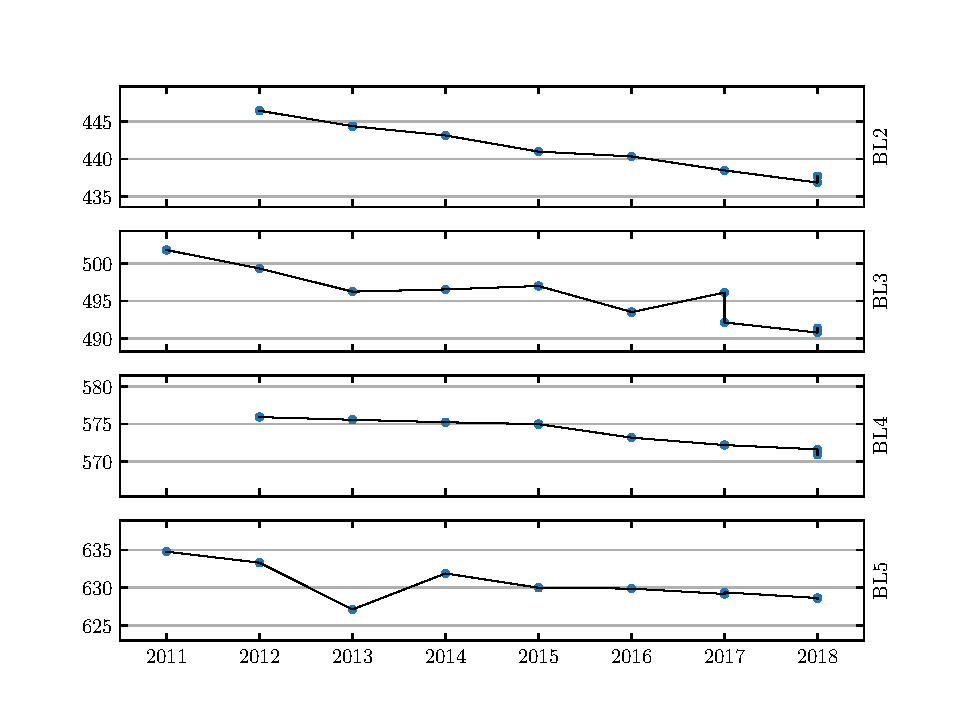
\includegraphics[width=\textwidth]{./figs/Elevation_Blekumbreen.pdf}
    \caption{capt.}
    \label{GPS:fig:elev_ble}
\end{figure}


\begin{figure}[H]
    \centering
    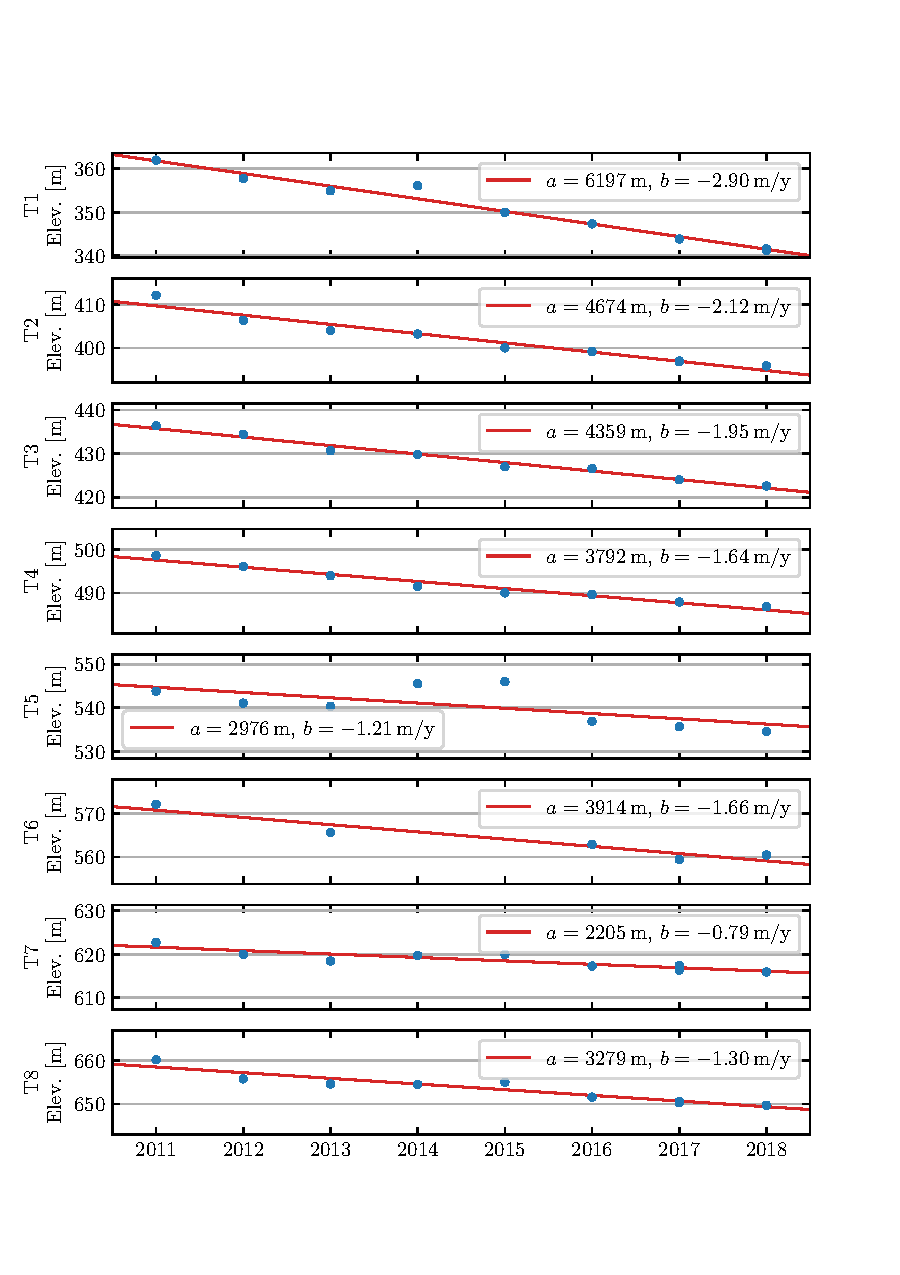
\includegraphics[width=\textwidth]{./figs/Elevation_Tellbreen.pdf}
    \caption{capt.}
    \label{GPS:fig:elev_tel}
\end{figure}